\documentclass[11pt,preprint, authoryear]{elsarticle}

\usepackage{lmodern}
%%%% My spacing
\usepackage{setspace}
\setstretch{1.2}
\DeclareMathSizes{12}{14}{10}{10}

% Wrap around which gives all figures included the [H] command, or places it "here". This can be tedious to code in Rmarkdown.
\usepackage{float}
\let\origfigure\figure
\let\endorigfigure\endfigure
\renewenvironment{figure}[1][2] {
    \expandafter\origfigure\expandafter[H]
} {
    \endorigfigure
}

\let\origtable\table
\let\endorigtable\endtable
\renewenvironment{table}[1][2] {
    \expandafter\origtable\expandafter[H]
} {
    \endorigtable
}


\usepackage{ifxetex,ifluatex}
\usepackage{fixltx2e} % provides \textsubscript
\ifnum 0\ifxetex 1\fi\ifluatex 1\fi=0 % if pdftex
  \usepackage[T1]{fontenc}
  \usepackage[utf8]{inputenc}
\else % if luatex or xelatex
  \ifxetex
    \usepackage{mathspec}
    \usepackage{xltxtra,xunicode}
  \else
    \usepackage{fontspec}
  \fi
  \defaultfontfeatures{Mapping=tex-text,Scale=MatchLowercase}
  \newcommand{\euro}{€}
\fi

\usepackage{amssymb, amsmath, amsthm, amsfonts}

\def\bibsection{\section*{References}} %%% Make "References" appear before bibliography


\usepackage[round]{natbib}

\usepackage{longtable}
\usepackage[margin=2.3cm,bottom=2cm,top=2.5cm, includefoot]{geometry}
\usepackage{fancyhdr}
\usepackage[bottom, hang, flushmargin]{footmisc}
\usepackage{graphicx}
\numberwithin{equation}{section}
\numberwithin{figure}{section}
\numberwithin{table}{section}
\setlength{\parindent}{0cm}
\setlength{\parskip}{1.3ex plus 0.5ex minus 0.3ex}
\usepackage{textcomp}
\renewcommand{\headrulewidth}{0.2pt}
\renewcommand{\footrulewidth}{0.3pt}

\usepackage{array}
\newcolumntype{x}[1]{>{\centering\arraybackslash\hspace{0pt}}p{#1}}

%%%%  Remove the "preprint submitted to" part. Don't worry about this either, it just looks better without it:
\makeatletter
\def\ps@pprintTitle{%
  \let\@oddhead\@empty
  \let\@evenhead\@empty
  \let\@oddfoot\@empty
  \let\@evenfoot\@oddfoot
}
\makeatother

 \def\tightlist{} % This allows for subbullets!

\usepackage{hyperref}
\hypersetup{breaklinks=true,
            bookmarks=true,
            colorlinks=true,
            citecolor=blue,
            urlcolor=blue,
            linkcolor=blue,
            pdfborder={0 0 0}}


% The following packages allow huxtable to work:
\usepackage{siunitx}
\usepackage{multirow}
\usepackage{hhline}
\usepackage{calc}
\usepackage{tabularx}
\usepackage{booktabs}
\usepackage{caption}


\newenvironment{columns}[1][]{}{}

\newenvironment{column}[1]{\begin{minipage}{#1}\ignorespaces}{%
\end{minipage}
\ifhmode\unskip\fi
\aftergroup\useignorespacesandallpars}

\def\useignorespacesandallpars#1\ignorespaces\fi{%
#1\fi\ignorespacesandallpars}

\makeatletter
\def\ignorespacesandallpars{%
  \@ifnextchar\par
    {\expandafter\ignorespacesandallpars\@gobble}%
    {}%
}
\makeatother

\newlength{\cslhangindent}
\setlength{\cslhangindent}{1.5em}
\newenvironment{CSLReferences}%
  {\setlength{\parindent}{0pt}%
  \everypar{\setlength{\hangindent}{\cslhangindent}}\ignorespaces}%
  {\par}


\urlstyle{same}  % don't use monospace font for urls
\setlength{\parindent}{0pt}
\setlength{\parskip}{6pt plus 2pt minus 1pt}
\setlength{\emergencystretch}{3em}  % prevent overfull lines
\setcounter{secnumdepth}{5}

%%% Use protect on footnotes to avoid problems with footnotes in titles
\let\rmarkdownfootnote\footnote%
\def\footnote{\protect\rmarkdownfootnote}
\IfFileExists{upquote.sty}{\usepackage{upquote}}{}

%%% Include extra packages specified by user
\usepackage{booktabs}
\usepackage{longtable}
\usepackage{array}
\usepackage{multirow}
\usepackage{wrapfig}
\usepackage{float}
\usepackage{colortbl}
\usepackage{pdflscape}
\usepackage{tabu}
\usepackage{threeparttable}
\usepackage{threeparttablex}
\usepackage[normalem]{ulem}
\usepackage{makecell}
\usepackage{xcolor}

%%% Hard setting column skips for reports - this ensures greater consistency and control over the length settings in the document.
%% page layout
%% paragraphs
\setlength{\baselineskip}{12pt plus 0pt minus 0pt}
\setlength{\parskip}{12pt plus 0pt minus 0pt}
\setlength{\parindent}{0pt plus 0pt minus 0pt}
%% floats
\setlength{\floatsep}{12pt plus 0 pt minus 0pt}
\setlength{\textfloatsep}{20pt plus 0pt minus 0pt}
\setlength{\intextsep}{14pt plus 0pt minus 0pt}
\setlength{\dbltextfloatsep}{20pt plus 0pt minus 0pt}
\setlength{\dblfloatsep}{14pt plus 0pt minus 0pt}
%% maths
\setlength{\abovedisplayskip}{12pt plus 0pt minus 0pt}
\setlength{\belowdisplayskip}{12pt plus 0pt minus 0pt}
%% lists
\setlength{\topsep}{10pt plus 0pt minus 0pt}
\setlength{\partopsep}{3pt plus 0pt minus 0pt}
\setlength{\itemsep}{5pt plus 0pt minus 0pt}
\setlength{\labelsep}{8mm plus 0mm minus 0mm}
\setlength{\parsep}{\the\parskip}
\setlength{\listparindent}{\the\parindent}
%% verbatim
\setlength{\fboxsep}{5pt plus 0pt minus 0pt}



\begin{document}



\begin{frontmatter}  %

\title{Question 4}

% Set to FALSE if wanting to remove title (for submission)




\author[Add1]{Joshua Strydom\footnote{\textbf{Contributions:}
  \newline \emph{The authors would like to thank no institution for
  money donated to this project. Thank you sincerely.}}}
\ead{20718284@sun.ac.za}





\address[Add1]{Stellenbosch University, Stellenbosch, South Africa}



\vspace{1cm}





\vspace{0.5cm}

\end{frontmatter}



%________________________
% Header and Footers
%%%%%%%%%%%%%%%%%%%%%%%%%%%%%%%%%
\pagestyle{fancy}
\chead{}
\rhead{}
\lfoot{}
\rfoot{\footnotesize Page \thepage}
\lhead{}
%\rfoot{\footnotesize Page \thepage } % "e.g. Page 2"
\cfoot{}

%\setlength\headheight{30pt}
%%%%%%%%%%%%%%%%%%%%%%%%%%%%%%%%%
%________________________

\headsep 35pt % So that header does not go over title




\hypertarget{introduction}{%
\section{\texorpdfstring{Introduction
\label{Introduction}}{Introduction }}\label{introduction}}

I previously calculated the full daily return of the ALSI by summing the
returns per day from each constituent stock in Question 3. I will
continue to make use of this data.

\begin{figure}[H]

{\centering \includegraphics{Question4_files/figure-latex/Figure1-1} 

}

\caption{ALSI cumulative returns \label{Figure1}}\label{fig:Figure1}
\end{figure}

Figure \ref{Figure1} above displays the cumulative return of the ALSI.

\hypertarget{principal-component-analysis}{%
\section{\texorpdfstring{Principal Component Analysis
\label{PCA}}{Principal Component Analysis }}\label{principal-component-analysis}}

\begin{figure}[H]

{\centering \includegraphics{Question4_files/figure-latex/Figure2-1} 

}

\caption{Eigenvalue proportions \label{Figure2}}\label{fig:Figure2}
\end{figure}

Figure \ref{Figure2} says that nearly 55\% of variation in the sectors
are explained by a single component. The eigenvectors can be interpreted
as the loadings or the weights of each PC. I will now look at the first
two PC's loadings so that I can make an interesting observation.

\begin{figure}[H]

{\centering \includegraphics{Question4_files/figure-latex/Figure3-1} 

}

\caption{Eigenvector proportions \label{Figure3}}\label{fig:Figure3}
\end{figure}

I noted from the eigenvalues that a unique linear combination of all the
sector returns can explain roughly 55\% of the variation in the returns
series. From Figure \ref{Figure3} above, I note that this unique
combination does not have an equal weighted input for the series.

\begin{figure}[H]

{\centering \includegraphics{Question4_files/figure-latex/Figure4-1} 

}

\caption{Eigenvector proportions \label{Figure4}}\label{fig:Figure4}
\end{figure}

From Figure \ref{Figure4}, I note that the second eigenvalue (which
explains about 27\% of the total variation) loads nearly equally on AGL
and BHP in the same direction but loads heavily on NPN in the opposite
direction. This implies (loosely) that holding a long AGL and BHP
position and a short NPN position explains a sizeable part of the total
variation in these sectors' overall returns.

\begin{figure}[H]

{\centering \includegraphics{Question4_files/figure-latex/Figure5-1} 

}

\caption{PCA variables \label{Figure5}}\label{fig:Figure5}
\end{figure}

Figure \ref{Figure5} shows the relationship between all variables.
Positively correlated variables are grouped together. The distance
between variables and the origin measures the quality of the variables
on the factor map. Variables that are away from the origin are well
represented on the factor map. The closer a variable is to the unit
circle of correlations, the better its representation on the factor map
(and the more important it is to interpret these components)

\begingroup\fontsize{12pt}{13pt}\selectfont
\begin{longtable}{rrrrr}
\caption{Contributions of variables} \\ 
  \toprule
Dim.1 & Dim.2 & Dim.3 & Dim.4 & Dim.5 \\ 
  \hline 
\endhead 
\hline 
{\footnotesize Continued on next page} 
\endfoot 
\endlastfoot 
 \midrule
9.21 & 7.70 & 3.31 & 0.03 & 3.89 \\ 
  5.51 & 21.64 & 6.52 & 0.22 & 5.22 \\ 
  5.55 & 24.07 & 4.19 & 0.57 & 3.50 \\ 
  2.70 & 8.94 & 19.36 & 0.00 & 4.43 \\ 
  9.81 & 7.52 & 1.46 & 0.35 & 1.38 \\ 
  9.48 & 0.38 & 9.88 & 20.73 & 0.07 \\ 
  9.06 & 0.35 & 13.62 & 21.39 & 0.51 \\ 
  5.25 & 0.16 & 2.60 & 1.24 & 64.56 \\ 
  9.53 & 7.19 & 1.81 & 0.00 & 2.21 \\ 
  2.15 & 0.04 & 26.75 & 50.39 & 5.07 \\ 
  7.96 & 0.95 & 0.20 & 2.02 & 8.18 \\ 
  10.29 & 3.89 & 3.23 & 0.02 & 0.48 \\ 
  8.28 & 4.45 & 0.80 & 2.14 & 0.37 \\ 
  5.20 & 12.73 & 6.27 & 0.91 & 0.14 \\ 
   \bottomrule
\end{longtable}
\endgroup

The above table shows the contribution of the variables. I will now
provide a visual representation of this.

\begin{figure}[H]

{\centering \includegraphics{Question4_files/figure-latex/Figure6-1} 

}

\caption{Contributions \label{Figure6}}\label{fig:Figure6}
\end{figure}

Figure \ref{Figure6} displays the total contribution of the stocks on
PC1 and PC2.

\hypertarget{dimension-description}{%
\section{Dimension description}\label{dimension-description}}

\begingroup\fontsize{12pt}{13pt}\selectfont
\begin{longtable}{lll}
\caption{Dimension description} \\ 
  \toprule
Tickers & correlation & p.value \\ 
  \hline 
\endhead 
\hline 
{\footnotesize Continued on next page} 
\endfoot 
\endlastfoot 
 \midrule
SBK & 0.8077564 & 0.000000e+00 \\ 
  FSR & 0.7887572 & 0.000000e+00 \\ 
  NED & 0.7771412 & 0.000000e+00 \\ 
  INL & 0.7754290 & 0.000000e+00 \\ 
  ABG & 0.7642331 & 0.000000e+00 \\ 
  INP & 0.7578773 & 0.000000e+00 \\ 
  SLM & 0.7245234 & 0.000000e+00 \\ 
  REM & 0.7105047 & 0.000000e+00 \\ 
  BHP & 0.5932059 & 0.000000e+00 \\ 
  AGL & 0.5912447 & 0.000000e+00 \\ 
  MTN & 0.5766738 & 9.205497e-306 \\ 
  SOL & 0.5741416 & 1.719383e-302 \\ 
  CFR & 0.4138740 & 3.260387e-143 \\ 
  NPN & 0.3695124 & 2.461847e-112 \\ 
   \bottomrule
\end{longtable}
\endgroup

\hypertarget{rolling-constituent-correlation}{%
\section{\texorpdfstring{Rolling constituent correlation
\label{roll}}{Rolling constituent correlation }}\label{rolling-constituent-correlation}}

\begin{figure}[H]

{\centering 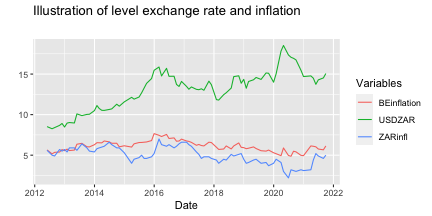
\includegraphics{Question4_files/figure-latex/Figure7-1} 

}

\caption{Pairwise correlations \label{Figure7}}\label{fig:Figure7}
\end{figure}

Figure \ref{Figure7} displays the pairwise correlations of the variables
under study.

\hypertarget{stratification}{%
\section{\texorpdfstring{Stratification
\label{strat}}{Stratification }}\label{stratification}}

\begingroup\fontsize{12pt}{13pt}\selectfont
\begin{longtable}{lrrlr}
\caption{Stratification of variables} \\ 
  \toprule
Tickers & SD & Full\_SD & Period & Ratio \\ 
  \hline 
\endhead 
\hline 
{\footnotesize Continued on next page} 
\endfoot 
\endlastfoot 
 \midrule
BHP & 0.07 & 0.04 & High\_Vol & 1.60 \\ 
  AGL & 0.06 & 0.04 & High\_Vol & 1.72 \\ 
  NPN & 0.05 & 0.04 & High\_Vol & 1.25 \\ 
  MTN & 0.03 & 0.02 & High\_Vol & 1.47 \\ 
  SOL & 0.03 & 0.02 & High\_Vol & 1.56 \\ 
  SAB & 0.03 & 0.02 & High\_Vol & 1.15 \\ 
  CFR & 0.03 & 0.02 & High\_Vol & 1.20 \\ 
  IMP & 0.02 & 0.01 & High\_Vol & 1.74 \\ 
  SBK & 0.02 & 0.01 & High\_Vol & 1.47 \\ 
  PRX & 0.02 & 0.01 & High\_Vol & 1.27 \\ 
  ANG & 0.01 & 0.01 & High\_Vol & 1.54 \\ 
  SSW & 0.01 & 0.01 & High\_Vol & 1.23 \\ 
  GFI & 0.01 & 0.01 & High\_Vol & 1.53 \\ 
  AMS & 0.01 & 0.01 & High\_Vol & 1.82 \\ 
  OML & 0.01 & 0.01 & High\_Vol & 1.51 \\ 
  FSR & 0.01 & 0.01 & High\_Vol & 1.36 \\ 
  BTI & 0.01 & 0.01 & High\_Vol & 1.30 \\ 
  HAR & 0.01 & 0.00 & High\_Vol & 1.44 \\ 
  MNP & 0.01 & 0.00 & High\_Vol & 1.57 \\ 
  SLM & 0.01 & 0.01 & High\_Vol & 1.22 \\ 
  ABG & 0.01 & 0.00 & High\_Vol & 1.37 \\ 
  ACL & 0.01 & 0.00 & High\_Vol & 1.45 \\ 
  REM & 0.01 & 0.00 & High\_Vol & 1.28 \\ 
  NHM & 0.01 & 0.00 & High\_Vol & 1.13 \\ 
  OMU & 0.01 & 0.00 & High\_Vol & 1.20 \\ 
  NPH & 0.01 & 0.00 & High\_Vol & 1.10 \\ 
  TKG & 0.01 & 0.00 & High\_Vol & 1.21 \\ 
  BID & 0.01 & 0.00 & High\_Vol & 1.13 \\ 
  SNH & 0.00 & 0.01 & High\_Vol & 0.92 \\ 
  MUR & 0.00 & 0.00 & High\_Vol & 1.00 \\ 
  ITU & 0.00 & 0.00 & High\_Vol & 1.71 \\ 
  CPI & 0.00 & 0.00 & High\_Vol & 1.41 \\ 
  SHP & 0.00 & 0.00 & High\_Vol & 1.14 \\ 
  BVT & 0.00 & 0.00 & High\_Vol & 1.21 \\ 
  APN & 0.00 & 0.00 & High\_Vol & 1.10 \\ 
  AEG & 0.00 & 0.00 & High\_Vol & 1.00 \\ 
  KIO & 0.00 & 0.00 & High\_Vol & 1.30 \\ 
  NED & 0.00 & 0.00 & High\_Vol & 1.34 \\ 
  AXL & 0.00 & 0.00 & High\_Vol & 1.42 \\ 
  SAP & 0.00 & 0.00 & High\_Vol & 1.26 \\ 
  RMH & 0.00 & 0.00 & High\_Vol & 1.48 \\ 
  VOD & 0.00 & 0.00 & High\_Vol & 1.43 \\ 
  MRP & 0.00 & 0.00 & High\_Vol & 1.22 \\ 
  INP & 0.00 & 0.00 & High\_Vol & 1.36 \\ 
  CLS & 0.00 & 0.00 & High\_Vol & 1.20 \\ 
  BAT & 0.00 & 0.00 & High\_Vol & 1.17 \\ 
  MCG & 0.00 & 0.00 & High\_Vol & 1.18 \\ 
  WHL & 0.00 & 0.00 & High\_Vol & 1.00 \\ 
  MDC & 0.00 & 0.00 & High\_Vol & 1.54 \\ 
  PPC & 0.00 & 0.00 & High\_Vol & 1.13 \\ 
  ARI & 0.00 & 0.00 & High\_Vol & 1.64 \\ 
  GLN & 0.00 & 0.00 & High\_Vol & 1.04 \\ 
  TBS & 0.00 & 0.00 & High\_Vol & 1.20 \\ 
  DSY & 0.00 & 0.00 & High\_Vol & 1.22 \\ 
  RDF & 0.00 & 0.00 & High\_Vol & 1.28 \\ 
  GRT & 0.00 & 0.00 & High\_Vol & 1.25 \\ 
  NRP & 0.00 & 0.00 & High\_Vol & 1.26 \\ 
  TFG & 0.00 & 0.00 & High\_Vol & 1.18 \\ 
  MEI & 0.00 & 0.00 & High\_Vol & 0.91 \\ 
  RNI & 0.00 & 0.00 & High\_Vol & 1.20 \\ 
  BAW & 0.00 & 0.00 & High\_Vol & 1.00 \\ 
  REI & 0.00 & 0.00 & High\_Vol & 1.28 \\ 
  TRU & 0.00 & 0.00 & High\_Vol & 0.86 \\ 
  INL & 0.00 & 0.00 & High\_Vol & 1.46 \\ 
  N91 & 0.00 & 0.00 & High\_Vol & 1.00 \\ 
  NTC & 0.00 & 0.00 & High\_Vol & 0.87 \\ 
  LBH & 0.00 & 0.00 & High\_Vol & 1.30 \\ 
  SPP & 0.00 & 0.00 & High\_Vol & 1.31 \\ 
  LHC & 0.00 & 0.00 & High\_Vol & 1.05 \\ 
  IPL & 0.00 & 0.00 & High\_Vol & 0.78 \\ 
  RMI & 0.00 & 0.00 & High\_Vol & 1.03 \\ 
  LGL & 0.00 & 0.00 & High\_Vol & 1.00 \\ 
  EXX & 0.00 & 0.00 & High\_Vol & 1.03 \\ 
  MTM & 0.00 & 0.00 & High\_Vol & 0.86 \\ 
  LON & 0.00 & 0.00 & High\_Vol & 1.39 \\ 
  NY1 & 0.00 & 0.00 & High\_Vol & 1.00 \\ 
  CCO & 0.00 & 0.00 & High\_Vol & 1.41 \\ 
  MND & 0.00 & 0.00 & High\_Vol & 1.09 \\ 
  PIK & 0.00 & 0.00 & High\_Vol & 1.45 \\ 
  RES & 0.00 & 0.00 & High\_Vol & 0.32 \\ 
  FFB & 0.00 & 0.00 & High\_Vol & 0.81 \\ 
  FFA & 0.00 & 0.00 & High\_Vol & 1.02 \\ 
  ANH & 0.00 & 0.00 & High\_Vol &  \\ 
  MTH & 0.00 & 0.00 & High\_Vol &  \\ 
  QLT & 0.00 & 0.00 & High\_Vol &  \\ 
   \bottomrule
\end{longtable}
\endgroup

\hypertarget{conclusion}{%
\section{Conclusion}\label{conclusion}}

Returns for the ALSI and SWIX seem to be concentrated in the large caps
stocks.

\bibliography{Tex/ref}





\end{document}
